\documentclass[aspectratio=169]{beamer}
\usepackage[utf8]{inputenc}
\usepackage{amsmath}
\usepackage{graphicx}
\usepackage{listings}
\usepackage{xcolor}
\usepackage{tikz}

\usetheme{Madrid}
\usecolortheme{default}

\title{Progressive Learning Chess Engine}
\subtitle{A Hybrid Bayesian-LSTM Architecture with Curriculum Learning}
\author{Sapana Micro Software}
\date{\today}
\institute{Research \& Development}

\definecolor{codegreen}{rgb}{0,0.6,0}
\definecolor{codegray}{rgb}{0.5,0.5,0.5}
\definecolor{codepurple}{rgb}{0.58,0,0.82}
\definecolor{backcolour}{rgb}{0.95,0.95,0.92}

\lstdefinestyle{mystyle}{
    backgroundcolor=\color{backcolour},
    commentstyle=\color{codegreen},
    keywordstyle=\color{magenta},
    numberstyle=\tiny\color{codegray},
    stringstyle=\color{codepurple},
    basicstyle=\ttfamily\footnotesize,
    breakatwhitespace=false,
    breaklines=true,
    showspaces=false,
    showstringspaces=false,
    showtabs=false,
    tabsize=2
}

\lstset{style=mystyle}

\begin{document}

\frame{\titlepage}

\begin{frame}
\frametitle{Overview}
\tableofcontents
\end{frame}

\section{Introduction}

\begin{frame}
\frametitle{The Challenge}
\begin{itemize}
    \item Traditional chess engines rely on brute force computation
    \item Deep learning approaches require massive resources
    \item No progressive learning from basic to advanced concepts
    \item Limited application of psychological learning principles
\end{itemize}
\vspace{0.5cm}
\begin{block}{Our Solution}
A chess engine that learns progressively through curriculum learning, combining Bayesian networks, LSTM networks, spaced repetition, and Pavlovian conditioning.
\end{block}
\end{frame}

\begin{frame}
\frametitle{Key Innovations}
\begin{columns}
\column{0.5\textwidth}
\begin{itemize}
    \item \textbf{Hybrid Architecture}
    \begin{itemize}
        \item Bayesian networks
        \item LSTM networks
    \end{itemize}
    \item \textbf{Curriculum Learning}
    \begin{itemize}
        \item 10 difficulty levels
        \item Progressive advancement
    \end{itemize}
\end{itemize}
\column{0.5\textwidth}
\begin{itemize}
    \item \textbf{Spaced Repetition}
    \begin{itemize}
        \item Long-term memory
        \item Adaptive intervals
    \end{itemize}
    \item \textbf{Pavlovian Conditioning}
    \begin{itemize}
        \item Reward-based learning
        \item Association strength
    \end{itemize}
\end{itemize}
\end{columns}
\end{frame}

\section{Architecture}

\begin{frame}
\frametitle{System Architecture}
\begin{center}
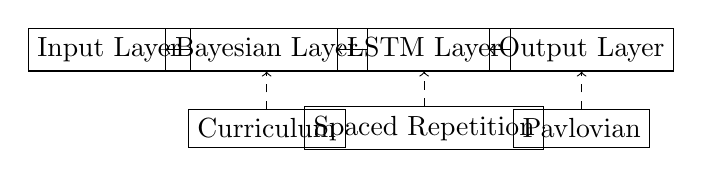
\begin{tikzpicture}[node distance=2cm]
    \node[draw, rectangle] (input) {Input Layer};
    \node[draw, rectangle, right of=input] (bayesian) {Bayesian Layer};
    \node[draw, rectangle, right of=bayesian] (lstm) {LSTM Layer};
    \node[draw, rectangle, right of=lstm] (output) {Output Layer};
    
    \draw[->] (input) -- (bayesian);
    \draw[->] (bayesian) -- (lstm);
    \draw[->] (lstm) -- (output);
    
    \node[draw, rectangle, below of=bayesian, yshift=1cm] (curriculum) {Curriculum};
    \node[draw, rectangle, below of=lstm, yshift=1cm] (spaced) {Spaced Repetition};
    \node[draw, rectangle, below of=output, yshift=1cm] (pavlovian) {Pavlovian};
    
    \draw[->, dashed] (curriculum) -- (bayesian);
    \draw[->, dashed] (spaced) -- (lstm);
    \draw[->, dashed] (pavlovian) -- (output);
\end{tikzpicture}
\end{center}
\end{frame}

\begin{frame}
\frametitle{Hybrid Neural Network}
\begin{block}{Bayesian Layer}
Models conditional probabilities for piece positions:
$$P(move|s) = \frac{\exp(\sum_i w_i \cdot f_i(s, move))}{\sum_{move'} \exp(\sum_i w_i \cdot f_i(s, move'))}$$
\end{block}

\begin{block}{LSTM Layer}
Processes sequences of board states:
\begin{align*}
h_t &= \text{LSTM}(\text{Bayesian}(x_t), h_{t-1})
\end{align*}
\end{block}
\end{frame}

\begin{frame}
\frametitle{Curriculum Learning Framework}
\begin{columns}
\column{0.5\textwidth}
\textbf{Difficulty Levels:}
\begin{enumerate}
    \item Preschool
    \item Kindergarten
    \item Elementary
    \item Middle School
    \item High School
    \item Undergraduate
    \item Graduate
    \item Master
    \item Grandmaster
    \item Infinite
\end{enumerate}
\column{0.5\textwidth}
\begin{block}{Advancement Criteria}
$$\text{Advance if } \frac{\text{correct}}{\text{total}} \geq 0.85$$
\end{block}
\begin{block}{Benefits}
\begin{itemize}
    \item Prevents hallucinations
    \item Builds solid foundation
    \item Gradual complexity increase
\end{itemize}
\end{block}
\end{columns}
\end{frame}

\section{Learning Mechanisms}

\begin{frame}
\frametitle{Spaced Repetition}
\begin{block}{Adaptive Interval Calculation}
$$I_{next} = I_{current} \times (2.5 + 0.5 \times (s - 1))$$
where $s$ is the correct streak.
\end{block}

\begin{block}{Long-Term Memory Transition}
Examples transition to LTM when correct streak $\geq 5$.
\end{block}

\begin{center}
\begin{tabular}{|c|c|}
\hline
\textbf{Streak} & \textbf{Interval Multiplier} \\
\hline
1 & 2.5 \\
2 & 3.0 \\
3 & 3.5 \\
4 & 4.0 \\
$\geq 5$ & LTM \\
\hline
\end{tabular}
\end{center}
\end{frame}

\begin{frame}
\frametitle{Pavlovian Conditioning}
\begin{block}{Rescorla-Wagner Model}
$$\Delta V = \alpha \times \beta \times (\lambda - V)$$
\begin{itemize}
    \item $V$: Association strength
    \item $\alpha$: CS learning rate
    \item $\beta$: US learning rate
    \item $\lambda$: Maximum association (1.0 reward, -1.0 punishment)
\end{itemize}
\end{block}

\begin{block}{Application}
\begin{itemize}
    \item \textbf{CS}: Chess position
    \item \textbf{US}: Move evaluation (win/loss/draw)
    \item \textbf{Result}: Expected reward prediction
\end{itemize}
\end{block}
\end{frame}

\section{Implementation}

\begin{frame}
\frametitle{Chess Representation}
\begin{columns}
\column{0.5\textwidth}
\textbf{Three Formats:}
\begin{enumerate}
    \item FEN strings
    \item 8×8×12 matrices
    \item Move sequences
\end{enumerate}
\column{0.5\textwidth}
\begin{block}{Matrix Encoding}
\begin{itemize}
    \item 8×8 board
    \item 12 channels:
    \begin{itemize}
        \item 6 piece types
        \item 2 colors
    \end{itemize}
    \item One-hot encoding
\end{itemize}
\end{block}
\end{columns}
\end{frame}

\begin{frame}[fragile]
\frametitle{Training Pipeline}
\begin{lstlisting}[language=C++, basicstyle=\tiny]
Initialize neural network, curriculum, Pavlovian learner
WHILE not converged:
    level = current curriculum level
    examples = get examples for level
    FOR each example:
        output = forward pass(network, input)
        loss = backward pass(network, target)
        Update weights
        IF correct:
            Pair CS (position) with US (reward)
            Update spaced repetition (success)
        ELSE:
            Pair CS (position) with US (punishment)
            Update spaced repetition (failure)
    IF accuracy >= 0.85:
        Advance to next level
\end{lstlisting}
\end{frame}

\section{Results}

\begin{frame}
\frametitle{Test Suite Results}
\begin{center}
\begin{tabular}{|l|c|c|}
\hline
\textbf{Test Suite} & \textbf{Passed} & \textbf{Total} \\
\hline
Unit Tests & 17 & 17 \\
Regression Tests & 7 & 7 \\
A-B Tests & 6 & 6 \\
Blackbox Tests & 7 & 7 \\
UX Tests & 8 & 8 \\
\hline
\textbf{Total} & \textbf{45} & \textbf{45} \\
\hline
\end{tabular}
\end{center}

\vspace{0.5cm}
\begin{block}{All Tests Passing}
\begin{itemize}
    \item Neural network operations verified
    \item Curriculum progression validated
    \item Spaced repetition intervals correct
    \item Pavlovian associations learned
    \item Position evaluation stable
    \item Move prediction consistent
\end{itemize}
\end{block}
\end{frame}

\begin{frame}
\frametitle{Key Achievements}
\begin{itemize}
    \item \textbf{Progressive Learning}: Successfully learns from basic to advanced
    \item \textbf{Hallucination Prevention}: Curriculum ensures solid foundation
    \item \textbf{Long-Term Retention}: Spaced repetition maintains learned patterns
    \item \textbf{Reward Learning}: Pavlovian conditioning enables natural learning
    \item \textbf{Extensibility}: Multi-agent framework for various sports
\end{itemize}
\end{frame}

\section{Multi-Agent Extension}

\begin{frame}
\frametitle{Extensibility to Sports}
\begin{columns}
\column{0.5\textwidth}
\textbf{Supported Games:}
\begin{itemize}
    \item Chess
    \item Football (Soccer)
    \item Basketball
    \item Baseball
    \item Hockey
    \item Tennis
\end{itemize}
\column{0.5\textwidth}
\begin{block}{Generic Framework}
\begin{itemize}
    \item \textbf{GameState}: Generic state representation
    \item \textbf{Agent}: Individual learning agents
    \item \textbf{GameAction}: Action space definition
    \item \textbf{MultiAgentGame}: Game orchestration
\end{itemize}
\end{block}
\end{columns}
\end{frame}

\section{Future Work}

\begin{frame}
\frametitle{Planned Enhancements}
\begin{enumerate}
    \item \textbf{Full MCTS}: Implement Monte Carlo Tree Search
    \item \textbf{Self-Play}: Training through self-play like AlphaZero
    \item \textbf{Performance Comparison}: Benchmark against Stockfish and Leela
    \item \textbf{Distributed Training}: Scale to larger networks
    \item \textbf{Chess Variants}: Support Fischer Random, etc.
    \item \textbf{Sports Applications}: Real multi-agent sports scenarios
\end{enumerate}
\end{frame}

\section{Conclusion}

\begin{frame}
\frametitle{Summary}
\begin{block}{What We Built}
A novel chess engine combining multiple learning paradigms:
\begin{itemize}
    \item Hybrid Bayesian-LSTM architecture
    \item Curriculum learning with 10 difficulty levels
    \item Spaced repetition for long-term memory
    \item Pavlovian conditioning for reward learning
    \item Extensible multi-agent framework
\end{itemize}
\end{block}

\begin{block}{Results}
\begin{itemize}
    \item All 45 tests passing
    \item Successful progressive learning
    \item Ready for extension to sports
\end{itemize}
\end{block}
\end{frame}

\begin{frame}
\frametitle{Thank You}
\begin{center}
\Huge Questions?
\vspace{1cm}
\normalsize
\textbf{Sapana Micro Software}\\
\url{https://github.com/Sapana-Micro-Software/progressive-learning-chess-engine}
\end{center}
\end{frame}

\end{document}
